\section{Design of the equalizer}
This chapter aims to describe the design of an digital equalizer, for an electric guitar. 
To begin with, some design choices have to made. From \autoref{tab:frequency_area} it is seen that the frequency area of an electric guitar is from \SI{80}{\hertz} to \SI{4400}{\hertz}. Thus the equalizer has to be able to change the frequency response in this area. This change in the frequency response is made by as series connection of shelving filters and peak filters. The shelving filters are used the highest and the lowest bands of the equalizer and the peak filters are used for the in between bands. All filters are normally kept as first or second order filters. 

\subsection{Shelving filter}
The transfer function for a second order normalized low shelving filter is as in \autoref{eq:analog_shelving_low}.

\begin{equation}\label{eq:analog_shelving_low}
        H_{norm}(s) = \frac{s^2+\sqrt{2 \cdot G} \cdot s + G}{s^2+\sqrt{2} \cdot s +1}
    \end{equation}

    \startexplain
     \explain{$G$ is the transition frequency between the high and the low frequency regions.}{\si{\radian/\second}}
    \stopexplain

 The transfer function is then scaled by setting $H_{LS}(s)=H_{norm}(\frac{s}{\omega_0})$, where $\omega_0$ is the wanted \SI{3}{\decibel} cut-off frequency. The high shelving filters can also be made from the normalized low shelving filter by setting $H_{HS}(s) = H_{norm}(\frac{\Omega_0}{s})$.

    
In \autoref{fig:low_and_high_shelving} a bodeplot of second order low- and high- shelving filters with different cut-off frequencies is shown.

\begin{figure}
    \centering
        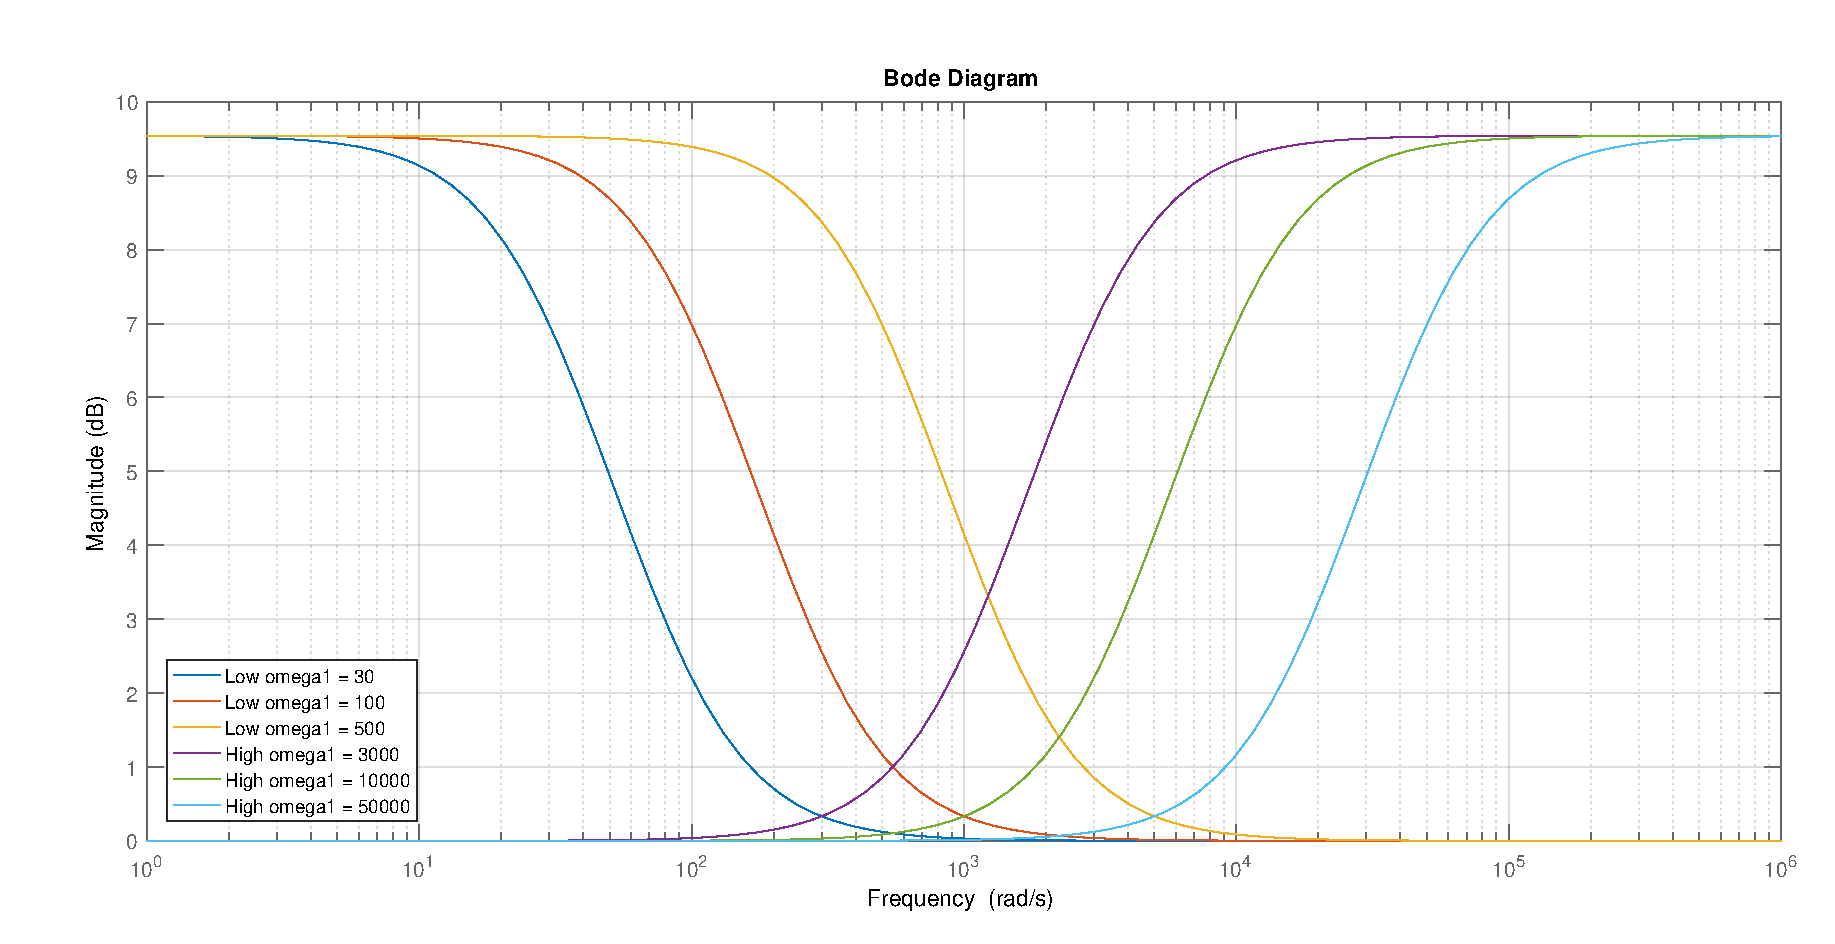
\includegraphics[width=\textwidth]{low_and_high_shelfing.pdf}
        \caption{Bodeplot of second order low- and high- shelving filters with different transition frequencies.}
        \label{fig:low_and_high_shelving}
  \end{figure} 
  \todo[inline]{figure is now first order}

\subsection{Peak filter}
The peak filters for the in between bands can be made from a number of design topologies. One of these are the constant-Q design. This design is sufficient the way that it keeps a specified bandwidth of the filter and therefore each individual filter's impact on the neighbouring filters can be controlled \citep{constant_Q}.
A way to make these constant-Q peak filters, and keep the order of the filter low, is by combining a second order lowpass filter with a high Q-value, and a linear function in Laplace domain.
The transfer function for the analog second order lowpass filter is as in \autoref{eq:analog_2nd_order_LP} and the transfer function for the analog linear function is as in \autoref{eq:analog_linear_function}. Their bodeplot can be seen in \autoref{fig:lin_function_&_2nd_order_LP}, where $Q = 4$ and $\omega_0 = 1000$. 

\begin{equation}\label{eq:analog_2nd_order_LP}
        H_{LP}(s) = \frac{\omega_0^2}{s^2+\frac{\omega_0}{Q}\cdot s + \omega_0^2}
    \end{equation}

    \startexplain
     \explain{$\omega_0$ is the cut-off frequency.}{\si{\radian/\second}}
     \explain{$Q$ is the ratio between the center frequency and the bandwidth.}{\si{1}}
    \stopexplain

\begin{equation}\label{eq:analog_linear_function}
        H_{lin}(s) = \frac{s}{\omega_0 \cdot Q}
    \end{equation}
    
\begin{figure}
    \centering
        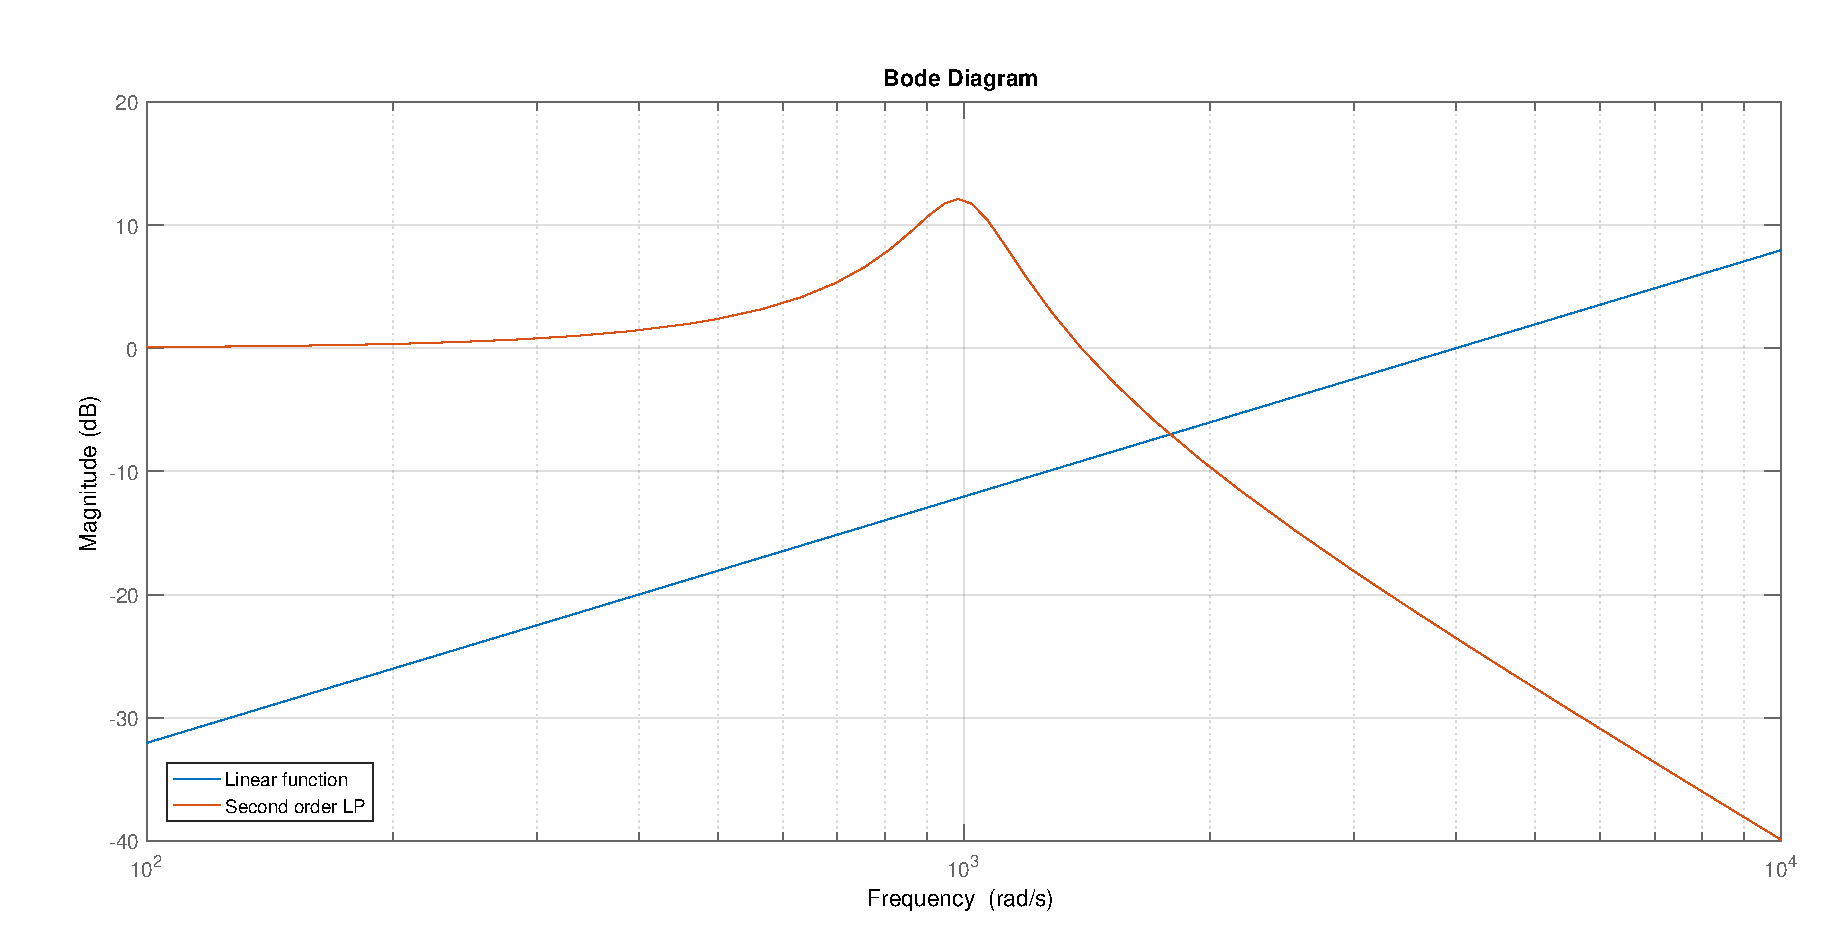
\includegraphics[width=\textwidth]{linear_function_and_2nd_order_LP.pdf}
        \caption{Bodeplot of a linear function and second order lowpass filter.}
        \label{fig:lin_function_&_2nd_order_LP}
  \end{figure} 

To make a peak filter, the two functions in \autoref{fig:lin_function_&_2nd_order_LP} are combined as illustrated the blockdiagram in \autoref{fig:peak_filter_block}.

\begin{figure}[!h]
\centering
\def\svgwidth{\columnwidth}
\input{figures/design/peak_filter_block.pdf_tex}
\caption{Block diagram of a peak filter.}
		\label{fig:peak_filter_block}
\end{figure}

When deriving the transfer function from \autoref{fig:peak_filter_block}, the transfer function for the peak filter is as in \autoref{eq:H_peak}, with a bodeplot as in \autoref{fig:peak_filter}, where $Q = 4$, $\omega_0 = 1000$ and various gain values. 

\begin{equation}\label{eq:H_peak}
        H_{peak}(s) = 1+G \cdot \frac{\frac{\omega_0}{Q}\cdot s}{s^2+\frac{\omega_0}{Q}\cdot s + \omega_0^2}
    \end{equation}
    
    \startexplain
     \explain{$G$ is the gain of the peak filter.}{\si{1}}
    \stopexplain

\begin{figure}[!h]
    \centering
        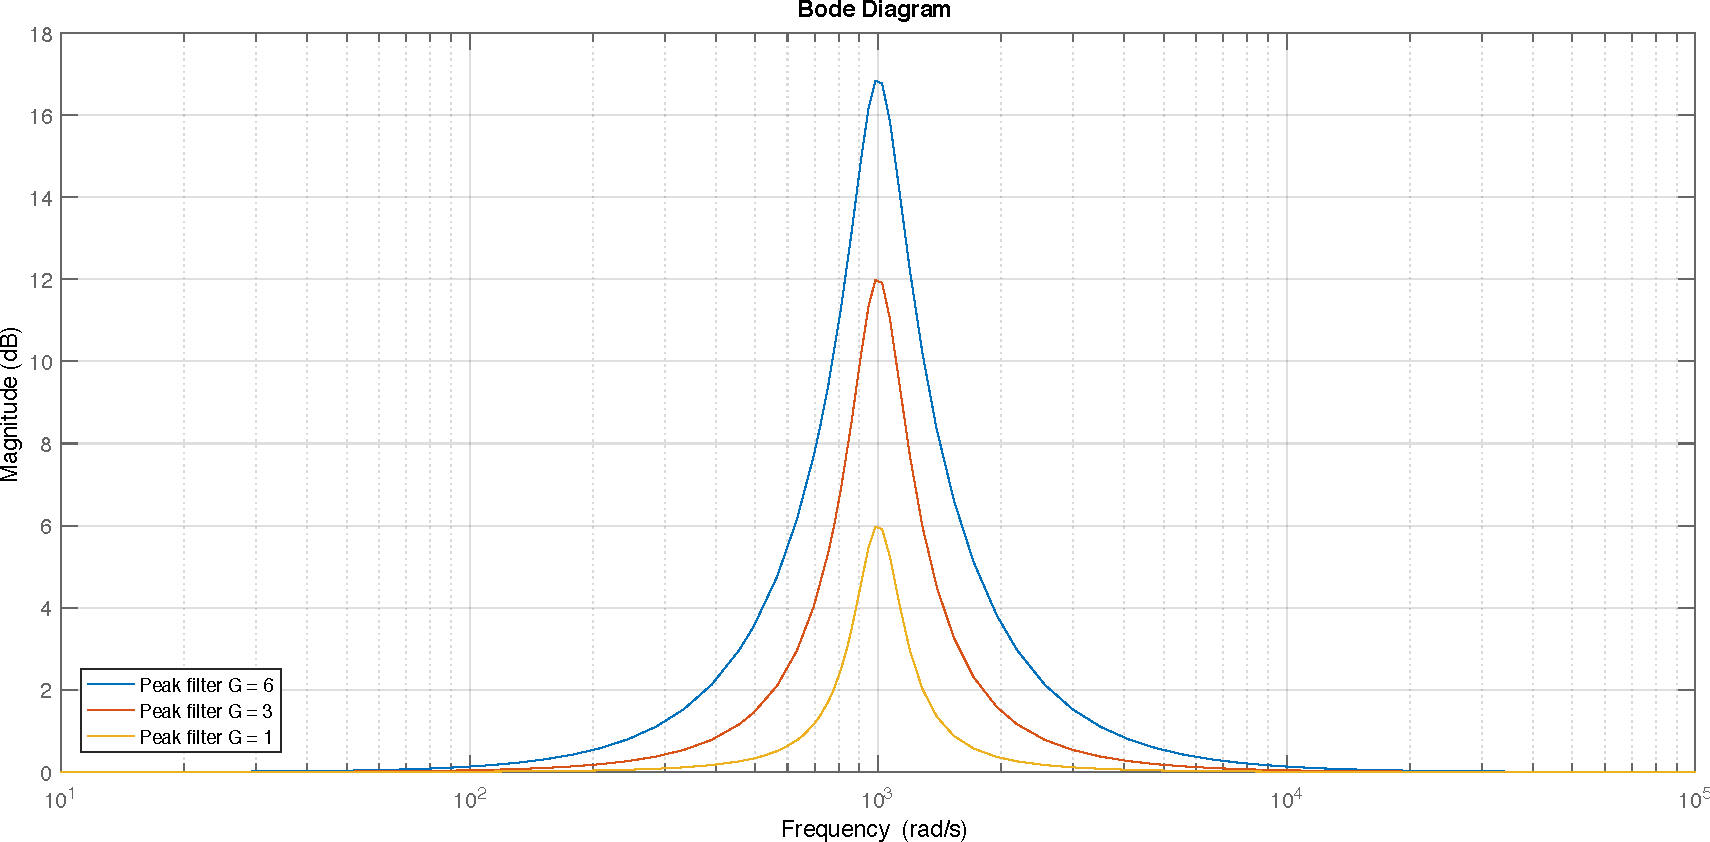
\includegraphics[width=\textwidth]{peak_filter.pdf}
        \caption{Bodeplot of a peak filter with various gain values.}
        \label{fig:peak_filter}
  \end{figure} 
  
\subsection{Design choices}
All the parts needed to make an equalizer have now been described. The parameters after which the equalizer shall be designed, will now be presented. 
The equalizer will be inspired by the BOSS GE-7 which is an analog equalizer for an electric guitar. The equalizer designed in this report will have the same number of bands and have the same attenuation and amplification ranges as the BOSS GE-7 \citep{Boss_GE7}. Thus the equalizer will have seven bands and be able to amplify each band $\pm$ \SI{15}{\decibel}.
The center frequencies of the 7 bands are also inspired by the BOSS GE-7 and is placed as in \autoref{tab:center_frequencies}.

\begin{table}[htbp]
\centering
\caption{Center frequencies for the equalizer.}
\label{tab:center_frequencies}
\begin{tabular}{|l|l|}
\cline{1-2}
\textbf{Band} & \textbf{Center frequency} \\ \cline{1-2}
1st & \SI{100}{\hertz} \\  \cline{1-2}
2nd & \SI{200}{\hertz}\\ \cline{1-2}
3rd & \SI{400}{\hertz} \\ \cline{1-2}
4th & \SI{800}{\hertz} \\ \cline{1-2}
5th & \SI{1600}{\hertz} \\ \cline{1-2}
6th & \SI{3200}{\hertz} \\ \cline{1-2}
7th & \SI{6400}{\hertz} \\ \cline{1-2}
\end{tabular}
\end{table}

The first and the seventh band will be made by shelving filters and band 2,3,4,5 and 6 will be made by peak filters. The aim of the design is to design an equalizer, where each band can be amplified $\pm$ \SI{15}{\decibel} and has a flat combined frequency response when each band is set to amplify \SI{15}{\decibel}.
The shelving filters will be designed first, followed by the peak filters. Since the cut-off frequencies, $\omega_0$ for the low shelving filter and $\Omega_0$ for the high shelving filter, are found in \autoref{tab:center_frequencies}, the only unknown in \autoref{eq:analog_shelving_low} is the gain, $G$.
The gain has to be changeable within $\pm$ \SI{15}{\decibel}. The gain value for a \SI{15}{\decibel} attenuation is found in \autoref{eq:shelving_gain_value}.

\begin{subequations}
\begin{equation}\label{eq:shelving_gain}
       20 \cdot \log_{10} \left(H_{norm}(j\cdot 1)\right) = 15 \addunit{\SI{}{\decibel}}
    \end{equation}
 \centering
$\Updownarrow$   
\begin{equation}\label{eq:shelving_gain_value}
       G = \mathopen|2.7328 + j5.0426\mathclose| = 5.73 \addunit{\SI{}{1}}
    \end{equation}
\end{subequations}

All parameters in the shelving filters are now known and the peak filters will now be designed.
Since $\omega_0$ is fixed for each band, only $G$ and $Q$ have to be determined. The gain, $G$, has to changeable within $\pm$ \SI{15}{\decibel}.
What the gain should be for the band to amplify \SI{15}{\decibel} is found in \autoref{eq:peak_gain_value}


\begin{subequations}
\begin{equation}\label{eq:peak_gain}
       20 \cdot \log_{10} \left(\mathopen|H_{peak}(j\omega_0)\mathclose|\right) = 20 \cdot \log_{10} \left(1+G\right) = 15 \addunit{\SI{}{\decibel}}
    \end{equation}
\centering
$\Updownarrow$
\begin{equation}\label{eq:peak_gain_value}
        G = -1+10^{\frac{3}{4}} = 4.62 \addunit{\SI{}{1}}
    \end{equation}
 \end{subequations}

The Q-value is then the only unknown in the design of the peak filters. In \autoref{req:bandpass_filter2} it is stated that at full amplification (\SI{15}{\decibel}), the amplification at $\omega = 1.5 \cdot \omega_0$ must diminished by one half (\SI{7.5}{\decibel}). The Q-value can be found by this relation and is calculated in \autoref{eq:peak_gain_value_half}

\begin{subequations}
\begin{equation}\label{eq:peak_gain_half}
       20 \cdot \log_{10} \left(H_{peak}(j\omega_0 \cdot 1.5)\right) = 7.5 \addunit{\SI{}{\decibel}}
    \end{equation}
\centering
$\Updownarrow$
\begin{equation}\label{eq:peak_gain_value_half}
        Q = \mathopen|j2.8456\mathclose| = 2.85 \addunit{\SI{}{1}}
    \end{equation}
 \end{subequations}
 
All parameters for the peak filters are then found. 



%Raised Cosine

%The interference effects on the side lying bandpass filter can easily be avoided by using an digital equalizer with third-octave raised cosine characteristics. The difference between the  bandpass filter characteristics and the one with a raised-cosine are shown in \autoref{fig:raised_cosine_vs_traditional}
%
%\begin{figure} [htbp]
% \centering
%  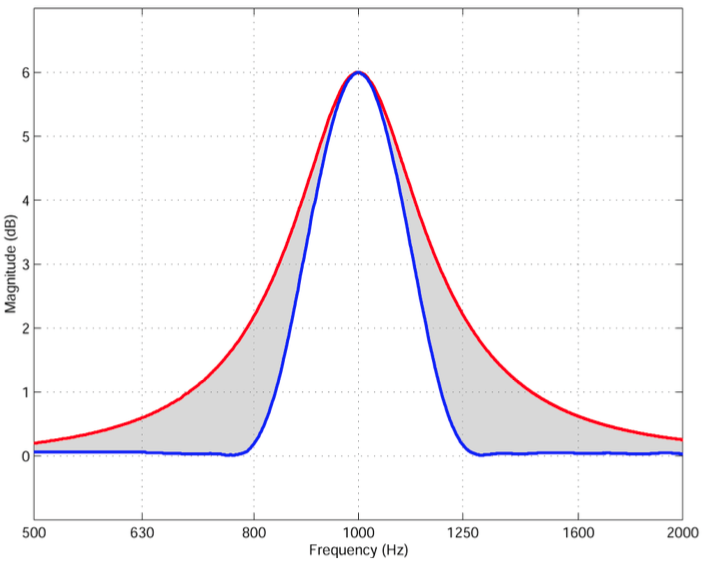
\includegraphics[width=0.7\textwidth]{raised_cosine_vs_traditional}
%  \caption{The photo shows the raised cosine bandpass filter characteristics versus traditional characteristics of third-octave bandpass filter \citep{nordic}
%  }
%  \label{fig:raised_cosine_vs_traditional}
%\end{figure}
%
%
%
%When using third-octave raised cosine bandpass filter, it is possible to make an equalizer where neighboring filters do not interfere with each other, or explained i another way, they interfere the right way, because a raised cosine filter does not leak into other third-octave bands like the traditional filter does. With this kind of filter it is possible to make a perfectly flat frequency response, and it is very close to an ideal equalizer. The \autoref{fig:raised_cosine_respond} shows the frequency response of a third-octave raised cosine equalizer designed by Dolby lake with the same gain and frequency settings as the analog equalizer at \autoref{fig:analog_equalizer}.
%
%\begin{figure} [htbp]
% \centering
%  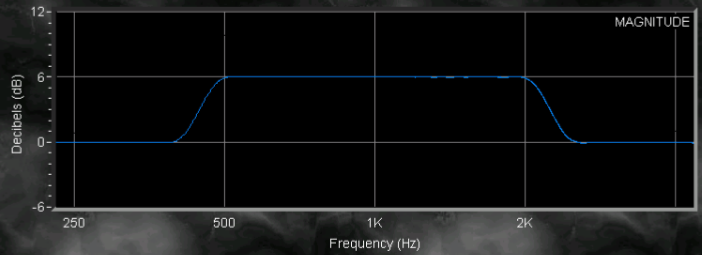
\includegraphics[width=0.8\textwidth]{raised_cosine_respond}
%  \caption{The photo shows an third-octave raised cosine equalizer frequency response  \citep{nordic}
%  }
%  \label{fig:raised_cosine_respond}
%\end{figure}
%
%
%The equalizer is used to compensate for the changes in sound due to different room characteristics, because the sound can be completely different in different rooms. The room characteristics will or can amplify or attenuate some frequency, and therefore the equalizer is very important to adjust the frequency in every new room.\citep{howtogeek} 
